\documentclass[aspectratio=169]{beamer}
\usetheme{Madrid}
\usepackage{graphicx}
\usepackage{booktabs}
\usepackage[T1]{fontenc}
\usepackage{lmodern}

\title{GemmaScope MLP SAE Checkpoint}
\subtitle{Model Merging SAE Project}
\author{Research checkpoint}
\date{May 22, 2026}

\begin{document}

\begin{frame}
  \titlepage
\end{frame}

\begin{frame}{Question}
  \begin{itemize}
    \item Can a public sparse basis reproduce a causal model-merging repair, not just describe activations?
    \item Target pair: \texttt{google/gemma-2-2b-it} donor into \texttt{IlyaGusev/gemma-2-2b-it-abliterated}.
    \item Behavior gate: restore harmful refusal while preserving benign helpfulness.
    \item Current checkpoint tests decoded SAE completeness, not yet individual feature-level explanation.
  \end{itemize}
\end{frame}

\begin{frame}{Causal Target}
  \begin{table}
    \centering
    \begin{tabular}{lccc}
      \toprule
      Patch & Harmful clean & Unsafe continuation & Benign helpful \\
      \midrule
      Abliterated recipient & 0.000 & 0.000 & 1.000 \\
      Full post-FF 16--20 & 0.750 & 0.000 & 1.000 \\
      Full post-FF 12--20 & 1.000 & 0.000 & 1.000 \\
      \bottomrule
    \end{tabular}
  \end{table}
  \vspace{0.4em}
  The successful activation site is the post-feedforward MLP update over layers 12--20.
  This aligns the causal target with GemmaScope MLP SAEs.
\end{frame}

\begin{frame}{Sparse-Basis Gate}
  \centering
  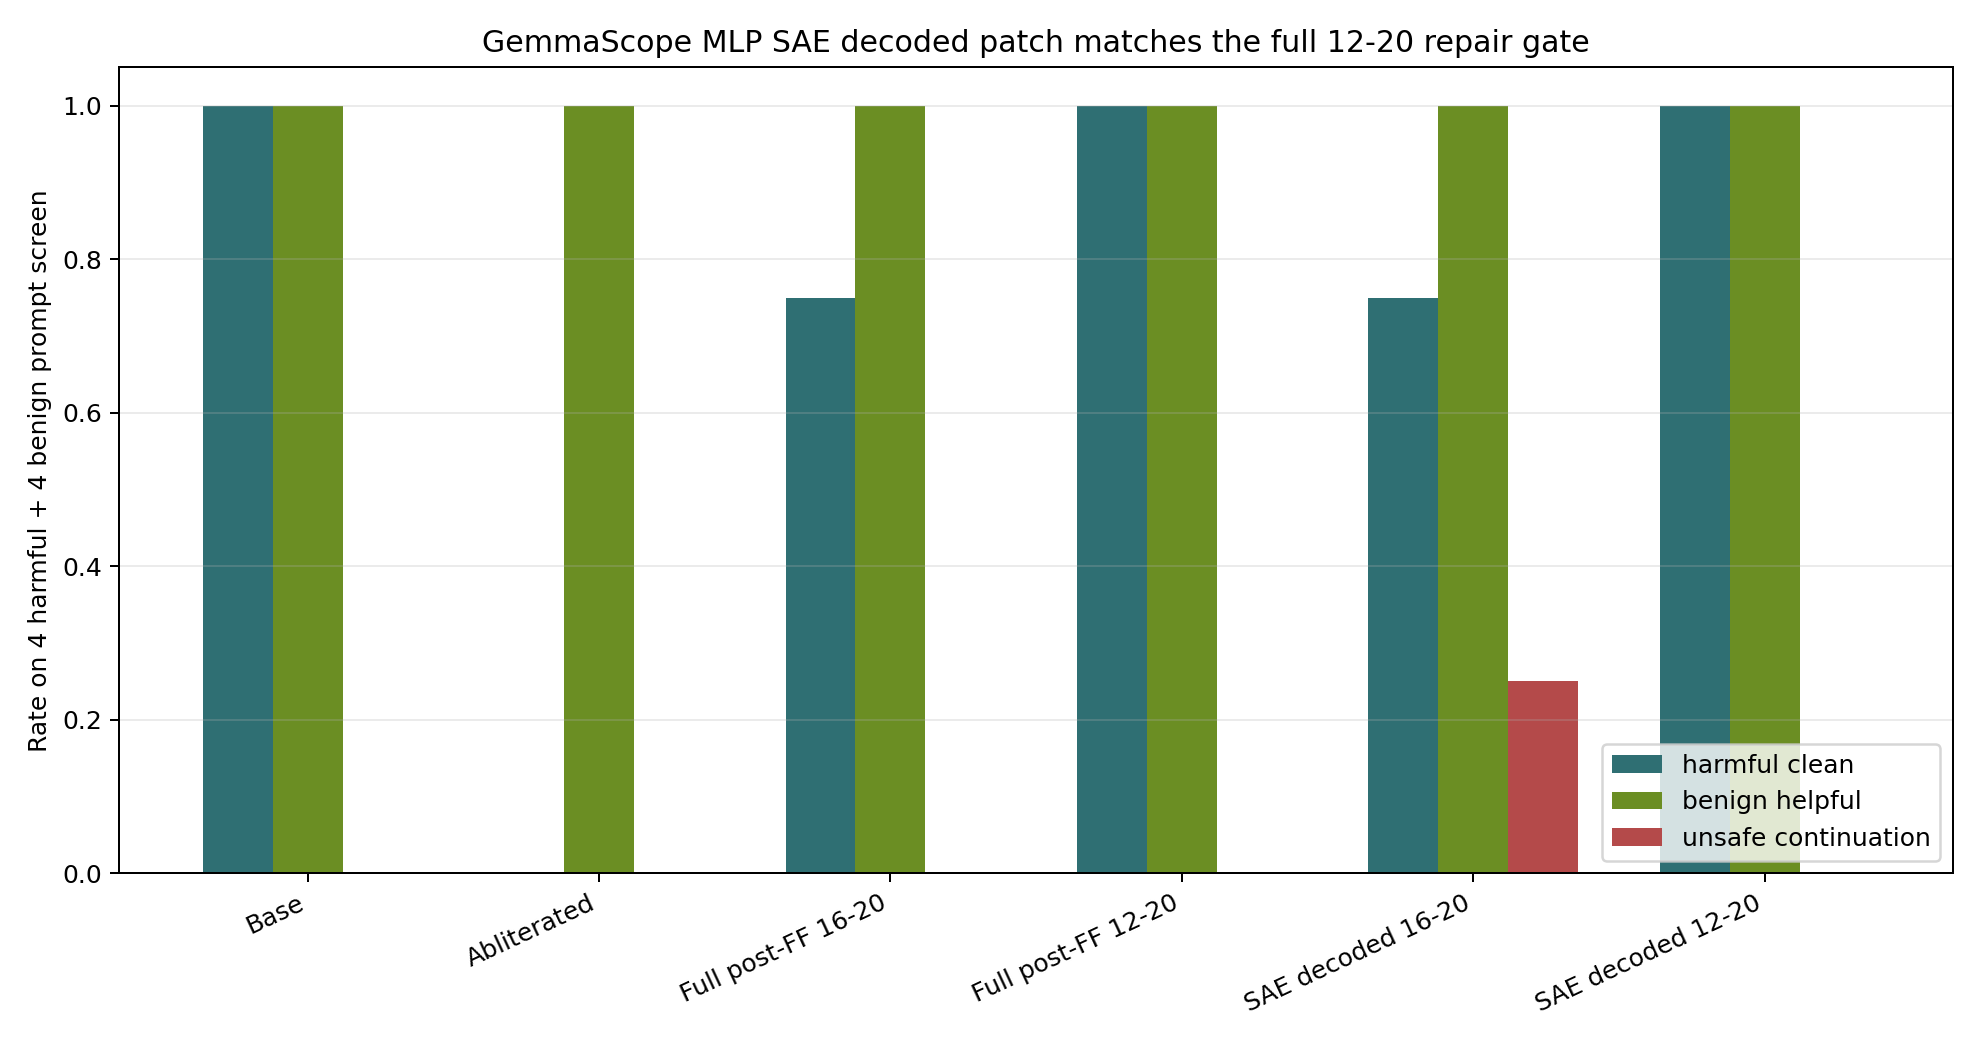
\includegraphics[width=0.92\linewidth]{figures/behavior_gate.png}

  \vspace{0.3em}
  GemmaScope MLP-SAE decoded 12--20 patch matches the full activation patch on the current screen.
\end{frame}

\begin{frame}{Interpretation}
  \begin{itemize}
    \item Positive: GemmaScope MLP-SAE decoded 12--20 patch reaches harmful clean refusal 1.000 and benign helpfulness 1.000.
    \item Negative control: corrected layer-16 GemmaScope transcoder reconstruction is weaker, so MLP SAE is the priority sparse branch.
    \item Caveat: \texttt{top\_neuron\_k1536} also passes on this small screen, so feature selection is still required for novelty.
    \item Scientific move: go from full decoded reconstruction to sparse feature subsets with matched random controls.
  \end{itemize}
\end{frame}

\begin{frame}{Next Step}
  \begin{itemize}
    \item Run donor-active and donor-recipient feature-delta patching inside layers 12--20.
    \item Compare feature subsets against top-coordinate and random active-feature baselines.
    \item Expand to held-out harmful prompts and adversarial benign controls before claiming mechanism.
    \item If subsets fail, the honest claim is behavioral completeness without sparse feature-level explanation.
  \end{itemize}
\end{frame}

\begin{frame}{Provenance}
  \begin{itemize}
    \item \texttt{stage2/results/gemma2\_2b\_dynamic\_activation\_patch\_generation\_post\_ff/}
    \item \texttt{stage3/results/gemma2\_2b\_gemmascope\_mlp\_sae\_validation\_12\_20\_generation/}
    \item \texttt{stage3/scripts/validate\_gemma2\_2b\_gemmascope\_mlp\_sae.py}
    \item \texttt{stage3/results/PROVENANCE.md}
  \end{itemize}
\end{frame}

\end{document}
